\cotefile{23}
\scanpage{83}
% manuscript lines 1
\uline{Lemme 1}

% manuscript lines 1–3
\margin{\uline{N\textsuperscript{o}} des \deleted{\unsure{Suit}} Rappels Sur la dimension}

% manuscript lines 1–3
\deleted{$A$ anneau local} $X$ préschéma \deleted{\unsure{loc.}} \unsure{noeth.|nœth.}, $Y$ partie fermée $\ne\varnothing$

% manuscript lines 4–5
\[
\begin{aligned}
(Y_i)_{i\in I}&\quad\text{ens des comp. irréductibles de }Y\\
(X_k)_{k\in K}&\quad\text{\rule{8em}{0.35pt} }X
\end{aligned}
\]

% manuscript lines 6
\[
\deleted{\unsure{I|J|\exists}}\quad r=\operatorname{Codim}(Y,X)
\]

% manuscript lines 7
$I'$ ens des $i\in I$ tels que $\operatorname{Codim}(Y_i,X)=r$

% manuscript lines 8–9
Pour $i\in I'$, $K_i=$ ens des $k\in K$ tels que \deleted{$\operatorname{codim}(\unsure{Y_i})$} $X_k\supset Y_i$ et $\operatorname{codim}(Y_i,X_k)=r$

% manuscript lines 10–11
Soit $x$ une section d'un Module inv. $\underline L$ sur $X$ telle que $V(x)\supset Y$. Alors,

% manuscript lines 12–15
$1^\circ)$ \inserted{On a} \deleted{\unsure{on a}} $\operatorname{Codim}(Y,V(x))\deleted{\unsure{>}}\unsure{\geq|>}r-1$ et pour qu'on ait égalité, il f. et s. qu'il existe $i\in I'$, $k\in K_i$ tels que $V(x)\not\supset X_k$. Pour ceci, il \uline{suffit} que \deleted{\unsure{rang}} $\unsure{\operatorname{Codim}|\operatorname{codim}}(V(x),X)\geq1$ \deleted{\unsure{quelque}} i.e. $=1$ \unsure{d'un}

% manuscript lines 16–20
$2^\circ)$ \deleted{Supposons $r>0$. Pour qu'on ait \uline{égalité} \unsure{quel que soit} \unsure{d'un} \unsure{A}} \inserted{Supposons que $X$ soit \deleted{\unsure{loc., fermé}} \unsure{ou quasi|un quasi} \unsure{affine} $X=V(\unsure{I|A})$, et $r>0$,} alors il existe un $x\in\unsure{\sqrt{I}|\sqrt{\mathfrak A}|\mathfrak A|\mathfrak m}$, tel que
\[
\left\{\begin{aligned}
\operatorname{Codim}(\deleted{\unsure{Y}}V(x),X)&=1\deleted{\unsure{4}},\quad\deleted{\unsure{\operatorname{Codim}(Y)}}\\
\text{et donc}\quad\deleted{\dim V(x)=\dim X-1}&\quad\operatorname{codim}(Y,V(x))=r-1 .
\end{aligned}\right.
\]
$X$ est local, on voit \deleted{\unsure{que}} \inserted{\unsure{prouve}} de plus $\dim V(x)=\dim X-1$

% manuscript lines 21
\uline{Dém} $1^\circ)$
\[
\operatorname{Codim}(Y,V(x))=\mathop{\mathrm{Inf}}\operatorname{Codim}(Y_i,V(x))\qquad\text{Or}
\]

% manuscript lines 22–23
\[
\begin{aligned}
\operatorname{Codim}(Y_i,V(x))&=\dim(\underline O_{V(x),y_i}\geq\dim(\underline O_{X,y_i}-1=\operatorname{Codim}(Y_i,X)-1\\
&\geq\operatorname{Codim}(Y,X)-1
\end{aligned}
\]

% manuscript lines 24
d'où
\[
\operatorname{Codim}(Y,V(x))\geq\operatorname{Codim}(Y,X)-1
\]

% manuscript lines 25–27
égalité ssi \deleted{\unsure{ssi}} \inserted{$\exists i$ tel qu'on} ait les deux égalités
\[
\left\{\begin{aligned}
\operatorname{Codim}(Y_i,V(x))&=\deleted{\dim}\operatorname{Codim}(Y_i,X)-1\\
\operatorname{Codim}(Y_i,X)&=\operatorname{Codim}(Y,X)
\end{aligned}\right.
\]
% archive sheet number: 82

\scanpage{84}
% manuscript lines 1
i.e. $i\in I'$, et $\exists k\in K_i$ t.q. $V(x)\supset X_k$.

% manuscript lines 2–5
$2^\circ)$ Comme $r>0$, pr ttes compos. irréd. $X_\alpha$ de $X$, on a $X_\alpha\not\subset Y$, donc \deleted{il existe $x\in\mathfrak A$ \unsure{tel déf.} que \unsure{Conséquence immédiate|Comme} pour que $I'\ne\varnothing$ et} $\mathfrak A\not\subset\mathfrak p_\alpha$, donc $\exists x'\in\mathfrak A$, $x\notin\bigcup_\alpha\mathfrak p_\alpha$.

% manuscript lines 6–12
% slanted
\margin{Il satisfait aux conditions envisagées}

% manuscript lines 6–12
\deleted{pour $i\in I'$, $K_i\ne\varnothing$, pour \unsure{de} \unsure{enfin} $r>0$ implique $X_k\supset Y_i$, $X_k\ne Y_i$, donc $X_k\not\subset Y$, donc $Y_i\not\supset X_k$, donc $Y_i\ne X_k$ $\exists x\in\mathfrak A$ t.q. $V(x)\unsure{\supset}$ $\mathfrak A\supset$ $\mathfrak p_k\not\supset\mathfrak A$, donc \unsure{conséquence} \unsure{des relations précédentes} $\mathfrak A\supsetneqq\mathfrak p$, donc $\exists x\in\mathfrak A$, $x\notin\mathfrak p$. $\exists x\in\mathfrak A$, $x\notin\mathfrak p_k$. De plus, pour ttes compos. irréductibles $X_{\deleted{\unsure{k}}\alpha}$ de $X$ de dim maximum, on a $X_\alpha\not\subset Y$ [sinon}

% manuscript lines 13–21
\uline{Corollaire 1} Soit $A$ anneau \inserted{local} noeth., \deleted{$X=\operatorname{Spec} A$, $Y=V(\mathfrak A)$ partie fermée de $X$,} $\mathfrak A$ \deleted{\unsure{un}} $\subset\deleted{\unsure{A}}A$ idéal, \deleted{$x\in\mathfrak A$} $r=\deleted{\operatorname{Codim}(Y,X)}\operatorname{ht}(\mathfrak A)$, alors il existe une \deleted{suite} $x_1\,\text{--}\,x_r$ d'éléments de $\mathfrak A$, \deleted{faisant partie d'un système de paramètres de $A$, et \unsure{alors} tels que $\operatorname{ht}(x_1,\text{--}x_r)$} avec $\operatorname{ht}(\sum x_i A)=r$, \deleted{et} \inserted{d'où} $\operatorname{ht}(\mathfrak A/(x_1,\text{--}x_r))=0$ ; si $A$ local, les $x_i$ font partie d'un syst. de paramètres. Prenant $\mathfrak A$ premier, on conclut

% manuscript lines 13–20
% margin note written sideways
\margin{\uline{Corollaire} Conditions équivalentes si $x_1,\text{--},x_p\in\unsure{\mathfrak r A|rA|\mathfrak m_A}$, $A$ local noeth. (i) $\operatorname{ht}(\sum A x_i)=p$ (on a tjs $\leq$) (ii) \deleted{pour tt} $x_1$ ne s'annule sur aucune comp. irréd de $\operatorname{Spec}(A)$, \ldots{} $x_{\unsure{n|r|p}}$ ne s'annule sur aucune comp. irréd de $\operatorname{Sp} A/\sum_1^{\unsure{n|r|p}-1}x_i A$}

% manuscript lines 22–27
\uline{Corollaire 2} Soit $\mathfrak p$ un idéal premier de $A$ local noeth, $r=\dim A_{\mathfrak p}$, Alors il existe $x_1\,\text{--}\,x_r\in\mathfrak p$ tels que les $x_i$ \deleted{\unsure{forment part|fassent part}} définissent un syst. de paramètres de $A_{\mathfrak p}$, et font partie d'un système de paramètres de $A/\mathfrak p$.
% archive sheet number: 83

\scanpage{85}
% manuscript lines 1
$\partial$-\uline{Catégorie} $\mathscr H$

% manuscript lines 2–6
\deleted{catégorie additive \uline{graduée}, i.e. où les $\operatorname{Hom}(X,Y)$ sont des groupes \uline{gradués} (la composition des morphismes étant additive sur les degrés), satisfaisant aux axiomes qui \deleted{vont} suivent. On désigne par $\mathscr H_{(0)}$ la catégorie $\mathscr H$ où les hom sont réduits au degré $0$.}

% manuscript lines 7–8
\deleted{\uline{Axiome} $\uline{\partial\,1}$ Pour tout $X\in\operatorname{Ob}\mathscr H$, il existe un \deleted{$\unsure{T}(Y)=Y(1)$} \deleted{$\unsure{T(Y)|X(1)}$} $\in\operatorname{Ob}\mathscr H$ et un isomorphisme fonctoriel \inserted{en $X$}, (sur $\mathscr H_{(0)}$) \deleted{en $X$}}

% manuscript lines 9
\[
\deleted{\operatorname{Hom}_1(X,Y)\overset{\sim}{\longrightarrow}\operatorname{Hom}_0(X,Y(1))}
\]

% manuscript lines 10
\deleted{Donc il y a un objet canonique}

% manuscript lines 11
\[
\deleted{i_Y\in\operatorname{Hom}_1(\deleted{\unsure{T}}\unsure{X(1)|T(Y)|Y(1)},Y)}
\]

% manuscript lines 12–13
\deleted{ayant une propriété universelle. Évidt \unsure{$(T(Y),i_Y)$|$(Y(1),i_Y)$} est défini à $\mathscr H_{(0)}$-isomorphisme près.}

% manuscript lines 14
\deleted{objet $X(1)$ de $\mathscr H$ et un \uline{isomorphisme} \uline{de degré $1$}}

% manuscript lines 15
\[
\deleted{\alpha_X:X(1)\underset{1}{\longrightarrow}X}
\]

% manuscript lines 16
\deleted{et un objet $X(-1)$ de $\mathscr H$ et un \uline{isomorphisme de degré $-1$}}

% manuscript lines 17
\[
\deleted{\beta_X:X(-1)\underset{-1}{\longrightarrow}X}
\]

% manuscript lines 18
\deleted{On en conclut, pour tt $Y$, des isomorphismes}

% manuscript lines 19–20
\[
\mathrm I\quad\left\{\begin{aligned}
\deleted{\operatorname{Hom}_n(X,Y)}&\deleted{\overset{\sim}{\longrightarrow}\operatorname{Hom}_{n+1}(X(1),Y)} .
\quad [=\operatorname{Hom}_{n-1}(X,\unsure{Y(1)})]\\
\deleted{\operatorname{Hom}_n(Y,X(1))}&\deleted{\unsure{=|\simeq|\overset{\sim}{\longrightarrow}}\operatorname{Hom}_{n+1}(Y,X)}
\end{aligned}\right.
\]

% manuscript lines 21–22
\[
\mathrm {II}\quad\left\{\begin{aligned}
\operatorname{Hom}_n(X,Y)&\overset{\sim}{\longrightarrow}\operatorname{Hom}_{n-1}(X(-1),Y)\\
\operatorname{Hom}_n(Y,X(-1))&\overset{\sim}{\longrightarrow}\operatorname{Hom}_{n-1}(Y,X)\deleted{\unsure{1}}
\end{aligned}\right.
\]
% archive sheet number: 84

\scanpage{87}
% manuscript lines 1–2
\deleted{\uline{\unsure{Déf.|Prop.}}} \uline{Lemme} Soient $A$ un anneau, $B$ une algèbre finie sur $A$, $M$ un $B$-mod de type fini.

% manuscript lines 3
(i) Si $M_{[A]}$ est $(S_k)$, il en est de $=$ de $M$

% manuscript lines 4–6
(ii) Supposons que pour \deleted{\unsure{tt}} idéaux premiers $\mathfrak q,\mathfrak q'$ de $B$, induisant \inserted{le $=$} $\mathfrak p$ sur $A$, on ait $\dim M_{\mathfrak q}=\dim M_{\mathfrak q'}$. Alors si $M$ est $(S_k)$ sur $B$, il est $(S_k)$ sur $A$.

% manuscript lines 7
On peut supposer $A\subset B$, \deleted{$\operatorname{Spec}\unsure{A|B}$} $\operatorname{Supp} M=\operatorname{Sp} B$

% manuscript lines 8–11
\uline{Dém} (i) Soit $\deleted{\unsure{\mathfrak p|\mathfrak q}}\mathfrak q\in\operatorname{Sp} A$, \deleted{si $\dim M_{\mathfrak p}\leq k$ \unsure{induisant} $\mathfrak q$ sur $A$, l'hypothèse indique que $\dim_{A_{\mathfrak q}}M_{\mathfrak q}=\dim_{B_{\mathfrak p}} M_{\mathfrak p}$, or \unsure{d'ailleurs} \unsure{par hypothèse}, on a $\operatorname{prof}$ [a fortiori $\dim_{A_{\mathfrak q}}M_{\mathfrak q}\geq\operatorname{Sup}_{\mathfrak p\,\mathrm{sur}\,\mathfrak q}\dim_{B_{\mathfrak p}}M_{\mathfrak p}$] et} on a

% manuscript lines 12
\[
\deleted{\text{si}}\quad \operatorname{prof}_{A_{\mathfrak q}} M_{\mathfrak q}=\mathop{\mathrm{Inf}}_{\mathfrak p\,\mathrm{sur}\,\mathfrak q}\operatorname{prof}_{B_{\mathfrak p}}M_{\mathfrak p},\quad
\deleted{\text{donc}}\quad \dim_{A_{\mathfrak q}}M_{\mathfrak q}=\mathop{\mathrm{Sup}}_{\mathfrak p\,\mathrm{sur}\,\mathfrak q}\dim_{B_{\mathfrak p}}M_{\mathfrak p}
\]

% manuscript lines 13
donc si $\mathfrak p$ sur $\mathfrak q$
\[
\operatorname{prof}_{B_{\mathfrak p}}M_{\mathfrak p}\geq\operatorname{prof}_{A_{\mathfrak q}}M_{\mathfrak q}\geq\operatorname{Inf}(k,\dim_{A_{\mathfrak q}}M_{\mathfrak q})\geq\operatorname{Inf}(k,\dim_{B_{\mathfrak p}}M_{\mathfrak p}),\quad\text{ck.}
\]

% manuscript lines 14–17
(ii) On a ici, grâce à l'hyp. spéciale
\[
\dim_{A_{\mathfrak q}}M_{\mathfrak q}=\dim_{A_{\mathfrak p}}M_{\mathfrak p}
\]
Or pour $\mathfrak p$ \uline{convenable} sur $\mathfrak q$, on aura \deleted{d'où \unsure{$M$} \unsure{si} \illegible{3} \unsure{l'occasion},}
\[
\deleted{\operatorname{prof}_{A_{\mathfrak q}}M_{\mathfrak q}\geq}\quad \operatorname{prof}_{A_{\mathfrak q}}M_{\mathfrak q}=\operatorname{prof}_{B_{\mathfrak p}}M_{\mathfrak p}\quad(\text{i.e. on a }{\geq})
\]

% manuscript lines 18–21
\deleted{Pour les \unsure{vérif.}, pour un système d'hyp\unsure{.} \unsure{sous} \illegible{2} et \unsure{chacun} de $\unsure{k\geq A_{\mathfrak q}|M_{\mathfrak q}}$, \unsure{en sorte, on est amené à} \unsure{trouver} qu'\unsure{elle} est aussi vérifiée pour} d'où le résultat voulu \textendash\ \textendash\ \textendash\ \textendash

% manuscript lines 22
$\deleted{\mathfrak p\subset\mathfrak q}$

% manuscript lines 22–23
\diagram{\begin{tikzcd}[ampersand replacement=\&,row sep=small,column sep=small]
\deleted{B}\&\deleted{M}\\
\deleted{A}\arrow[u,dash]\&\deleted{\unsure{\mathfrak p}}
\end{tikzcd}}

% manuscript lines 24
$\operatorname{prof}\geq\operatorname{Inf}(k,\dim)$

% manuscript lines 4–23
% margin note written sideways
\margin{$\unsure{\pi_1(Y)}\longrightarrow\unsure{\pi_1(X)}$ \unsure{$\psi$ bijective} \unsure{$x\in X$} $\unsure{\geq2}$ $\unsure{\geq3}$ \unsure{depth} $\unsure{\geq2}\Rightarrow\psi$ surj \unsure{depth} $\unsure{\geq3}$, \unsure{conditions} \illegible{2} $\Rightarrow\psi$ bij}

% manuscript lines 24
\figure{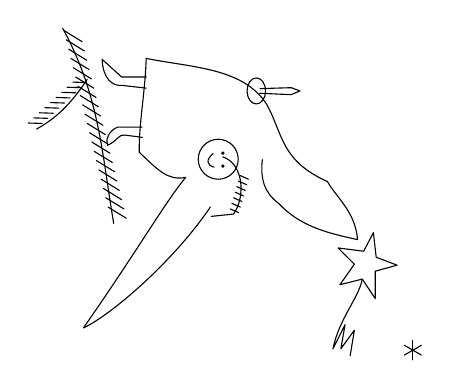
\begin{tikzpicture}[scale=.59,line cap=round,line join=round]
\begin{scope}[rotate=-90]
\draw (-2,0) .. controls (-1.8,1) and (-1.8,2.1) .. (-1,2.6) .. controls (-.35,2.95) and (.2,2.9) .. (.65,3.9) .. controls (1,4.1) and (1.3,4.5) .. (1.9,4.55) .. controls (1.75,3.85) and (1.6,3.3) .. (1.12,2.85) .. controls (.9,2.55) and (.6,2.45) .. (.18,2.5);
\draw (-2,0) .. controls (-1.2,-.03) and (-.6,-.16) .. (.02,-.15) .. controls (.4,.25) and (.64,.47) .. (.56,.85) .. controls (1.15,.37) and (2,-.1) .. (3.8,-1.35) .. controls (3.55,-.8) and (2.42,.55) .. (1.2,1.38);
\draw (-1.6,0)--(-1.6,-.53) .. controls (-1.8,-.75) and (-1.92,-.88) .. (-1.98,-.95) .. controls (-1.55,-.93) and (-1.4,-.72) .. (-1.42,-.52)--(-1.36,0);
\draw (-.52,-.09)--(-.52,-.62) .. controls (-.43,-.82) and (-.24,-.88) .. (-.13,-.83) .. controls (-.24,-.6) and (-.37,-.6) .. (-.35,-.46)--(-.3,-.08);
\draw (.12,1.65) .. controls (.27,2.1) and (.98,2.14) .. (1.35,1.88)--(1.4,1.4);
\draw (.17,1.55) circle (.43); \fill (.04,1.65) circle (.04) (.32,1.65) circle (.04); \draw (.05,1.44) .. controls (.18,1.28) and (.3,1.3) .. (.34,1.46);
\foreach \x in {0,...,6}{\draw (.52+.12*\x,2.02-.035*\x)--(.6+.12*\x,2.2-.035*\x);}
\draw (-1.3,2.37) ellipse (.28 and .2); \draw (-1.35,2.45)--(-1.37,3.12)--(-1.3,3.31)--(-1.22,3.12)--(-1.25,2.44);
\draw (2.45,5.4)--(2.58,4.93)--(3.17,4.93)--(2.75,4.65)--(2.87,4.17)--(2.43,4.48)--(2.08,4.13)--(2.15,4.68)--(1.75,4.89)--(2.28,4.95)--cycle;
\draw (2.75,4.65)..controls(3.15,4.58)and(3.6,4.15)..(4.25,4.02)--(3.73,4.28)--(4.25,4.19)--(3.85,4.48)--(4.4,4.39);
\foreach \a in {0,60,120}{\draw[shift={(4.28,5.74)},rotate=\a](-.21,0)--(.21,0);}
\draw (-2.65,-1.8)..controls(-1.2,-1)and(.1,-.95)..(1.55,-.7); \draw (-1.55,-1.27)..controls(-1.05,-1.6)and(-.72,-1.92)..(-.48,-2.36);
\foreach \i in {0,...,19}{\draw (-2.6+.2*\i,-1.77+.05*\i)--(-2.36+.2*\i,-1.38+.05*\i);}\foreach \i in {0,...,8}{\draw (-1.48+.11*\i,-1.28-.12*\i)--(-1.49+.11*\i,-1.58-.12*\i);}
\end{scope}\end{tikzpicture}}
% crop-candidate: scan 87
% archive sheet number: 86

\scanpage{88}
% manuscript lines 1–4
il s'ensuit que $\mathcal C$ est \uline{cohérent}. D'ailleurs, $\mathcal C$ satisfait $(S_2)$ en tout point de $Z$, car \deleted{si $x\in\unsure{Z}$, $V$ ouvert $\subset$ on a $\unsure{V|\mathcal M}\subset X$, on a $\Gamma(V,\mathcal C)\longrightarrow\Gamma(V\cap U,\mathcal C)$ est un isom.} par construction $\mathcal C\overset{\sim}{\longrightarrow}i_*\!i^*\mathcal C$.

% manuscript lines 4–9
Comme $\mathcal C\simeq B$ aux pts de $U$, \deleted{il s'} et que $B_x$ est une algèbre finie et normale sur $\underline O_{X,x}$, donc $(S_2)$ comme \unsure{anneau}, et par suite comme module, il s'ensuit que $\mathcal C$ est $(S_2)$ partout \inserted{comme Module,}. Celà \deleted{signifie} \unsure{signifie} aussi que l'anneau $C$ qui définit $\mathcal C$ est $S_2$. Bien \unsure{entendu} $A\subset C\subset K$.

% manuscript lines 5–9
% slanted
\margin{\unsure{Inutile} le fait que, $A$ étant quotient d'un régulier, on a $\dim A_{\mathfrak q}=\dim B_{\mathfrak p}$ si $\mathfrak p\in\operatorname{Spec} B$ induit $\mathfrak q$] cf verso}

% manuscript lines 9–18
Reste à prouver que $C$ est \deleted{\unsure{un|normal}} $(R_1)$. Soit $\mathfrak p$ un idéal premier de $C$ tel que $\dim C_{\mathfrak p}=1$, prouvons $C_{\mathfrak p}$ régulier. Soit $\mathfrak q$ l'idéal induit par $\mathfrak p$ sur $A$, alors [$A$ \deleted{est} quotient d'un régulier] on a $\dim A_{\mathfrak q}=1$, donc ou bien $A_{\mathfrak q}$ est normal, donc $A_{\mathfrak q}=B_{\mathfrak q}=B_{\mathfrak p}$ \deleted{\unsure{est donc}} normal, ou bien $A_{\mathfrak q}$ non normal, i.e. un des $\mathfrak p_i$, mais alors on a encore par construction $B_{\mathfrak q}$ normal, donc \deleted{$\unsure{B_{\mathfrak q}}$} $B_{\mathfrak p}$ est normal comme localisé de $B_{\mathfrak q}$. Celà achève la démonstration

% manuscript lines 19–23
\deleted{$A$ anneau (loclt noeth \unsure{par ex}), $B$ alg. finie sur $A$, \inserted{tt les idéaux \illegible{2}} $M$ module de type fini sur $B$, je dis que $M$ est $(S_n)$ sur $A$ ssi il est $(S_n)$ sur $B$. En \unsure{fait} supposons $A\subset B$, $\operatorname{Supp}M=\operatorname{Sp}B$, donc $f(X)=Y$. Soit $y\in Y$, on a $\operatorname{prof} M_y=\operatorname{Inf}_{z\,\mathrm{sur}\,y}\operatorname{prof}M_z$ \unsure{$\Rightarrow$} si $M$ sur $B$ est $(S_n)$, on a $\operatorname{prof}M_y\geq\operatorname{Inf}$}

% manuscript lines 22–23
\diagram{\begin{tikzcd}[ampersand replacement=\&,row sep=small]
f\&X\arrow[d]\\ \&Y
\end{tikzcd}}
% archive sheet number: 87

\scanpage{89}
% manuscript lines 1–4
\uline{Remarque} Soit $A$ un anneau intègre quotient d'un anneau régulier, $K$ son corps des fractions, \deleted{$L$ une extension finie de $K$,} Pour que la clôture intégre de $A$ soit de type fini, il f. et s. que $A$ satisfasse les conditions suivantes

% manuscript lines 5–6
a) L'ensemble des $\mathfrak p_i\in\operatorname{Spec} A$ tels que $A_{\mathfrak p_i}$ soit de dim $1$ \uline{non} \uline{régulier} est \uline{fini}

% manuscript lines 7–8
b) Pour tout tel $\mathfrak p_i\in\operatorname{Spec}(A)$, \deleted{tel que $\dim A_{\mathfrak p}=1$,} le normalisé de $A_{\mathfrak p}$ est fini \deleted{sur} $A_{\mathfrak p}$.

% manuscript lines 9–11
Dém. \uline{Nécessité évidente} [a) car le lieu \deleted{\unsure{singulier|régulier}} \inserted{non normal} de $\operatorname{Sp} A$ sera fermé, et les $\mathfrak p_i$ correspondent aux composantes irréd. de dim $1$ du dit]

% manuscript lines 12–16
\uline{Suffisance}. \deleted{Soit $B\subset K$ un \unsure{fini|finie} sur $A$, tel que les $B_{\mathfrak p_i}$ soient normaux [existe grâce à a), b)].} Comme $A$ est quotient d'un régulier, l'ens des $x\in\operatorname{Spec} A=X$ tels que $A_x$ soit $S_2$ est ouvert, et contient le pt générique \inserted{utilisant a) et le critère de Serre, on voit que $X_f$ \uline{normal},} il contient un ouvert non vide, soit $X_f$.

% manuscript lines 16–20
Il existe \deleted{\unsure{pour}} un sous-anneau $B\supset A$ de $K$, fini sur $A$, \deleted{tel que $B_f$ est} tel que \inserted{tt} $B_{\deleted{\unsure{f}}\mathfrak p_i}$ soit normal [utiliser a) et b)]. Soit $Z=\operatorname{Supp} B/A$, Alors $Z\subset X-X_f$, et $Z$ est de codim $>1$.

% manuscript lines 21–25
Soit $U=X-Z$, $i:U\longrightarrow X$ l'immersion canonique, $\mathscr B=\widetilde B$ faisceau d'alg. sur $X$, considérons \deleted{$\unsure{B|\mathcal B}$} $\mathcal C=i_*i^*(B)$. Comme le seul cycle \deleted{\unsure{immergé}} associé à $B$ est $X$, et que $Z$ est de codim $\geq2$ dans $X$, enfin $A$ quotient d'un régul\unsure{r.},
% archive sheet number: 88

\scanpage{90}
% manuscript lines 1–2
\diagram{\begin{tikzcd}[ampersand replacement=\&,row sep=tiny]
 B\arrow[d,dash,very thick]\&M\&\deleted{\text{Coh. Mac}}\\ A\&\&
\end{tikzcd}}

% manuscript lines 2
\[
\operatorname{prof}M_y\deleted{\leq}=\mathop{\mathrm{Inf}}_{z\leftrightarrow y}\operatorname{prof}M_z
\geq\mathop{\mathrm{Inf}}_z\deleted{\dim M_z,k}\operatorname{Inf}(\dim M_z,k)
\]

% manuscript lines 3
\deleted{$\unsure{M}$} \deleted{$M_y\leq$ \unsure{on ait} $\operatorname{Inf}$}

% manuscript lines 3–4
\diagram{\begin{tikzcd}[ampersand replacement=\&,row sep=tiny]
B\arrow[d,dash]\&\text{\uline{normal}}\\ A\&{}
\end{tikzcd}}

% manuscript lines 4–5
$S_2$ comme \deleted{\unsure{anneau}}, \unsure{anneau}, mais pas comme module

% manuscript lines 6
\[
 B/fB\simeq\unsure{0|O|\mathcal O}\,\unsure{0|{}_{X_0}}
\]

% manuscript lines 6–9
\figure{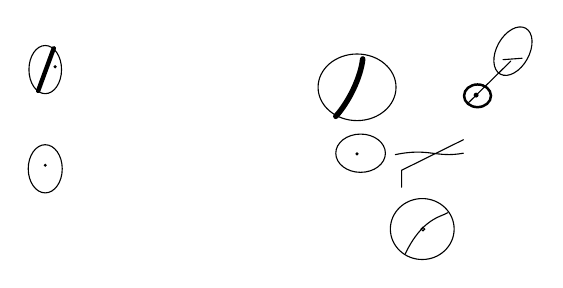
\begin{tikzpicture}[x=.9cm,y=.9cm,line cap=round]
\draw (0,2.9) ellipse (.23 and .34); \draw[line width=1.6pt](-.1,2.6)--(.12,3.2); \fill(.14,2.94)circle(.025);
\draw (0,1.5) ellipse (.24 and .34); \fill (0,1.55)circle(.023);
\draw (4.4,2.65) ellipse (.55 and .47); \draw[line width=2pt](4.1,2.24)..controls(4.28,2.44)and(4.45,2.78)..(4.48,3.05);
\draw (4.45,1.72) ellipse (.35 and .27); \fill (4.4,1.71)circle(.025);
\draw (5.32,.65) ellipse (.45 and .43); \draw (5.08,.3)..controls(5.32,.8)and(5.58,.82)..(5.68,.88); \draw(5.33,.65)circle(.025);
\draw (5.03,1.24)--(5.03,1.48)--(5.9,1.91); \draw(4.94,1.7)..controls(5.42,1.8)and(5.51,1.65)..(5.9,1.72);
\draw[line width=.9pt](6.1,2.53) ellipse (.19 and .16); \fill(6.08,2.54)circle(.035); \draw(5.97,2.43)--(6.57,3.02); \draw[rotate around={-29:(6.6,3.16)}](6.6,3.16) ellipse (.23 and .37); \draw(6.46,3.04)--(6.73,3.06);
\end{tikzpicture}}

% manuscript lines 7–9
\diagram{\begin{tikzcd}[ampersand replacement=\&,row sep=tiny]
B\arrow[d,dash,very thick]\&B\subset A^{\unsure{r|n}}\\
A\& A^n\qquad B/fB\subset(A/fA)^r
\end{tikzcd}}

% manuscript lines 9
\figure{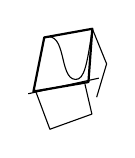
\begin{tikzpicture}[scale=.55,line join=round]
\draw[thick] (0,0)--(.25,1.25)--(1.36,1.45)--(1.27,.22)--cycle;
\draw (.04,.04)--(.38,-.87)--(1.35,-.52)--(1.19,.17); \draw (1.36,1.45)--(1.69,.64)--(1.46,-.13);
\draw (.25,1.25) .. controls (.78,1.42) and (.58,.3) .. (.97,.28) .. controls (1.18,.27) and (1.24,.64) .. (1.36,1.45);
\draw(-.12,-.05)--(1.51,.31);
\end{tikzpicture}}

% manuscript lines 10–11
\diagram{\begin{tikzcd}[ampersand replacement=\&,row sep=tiny]
B\arrow[d,dash,very thick]\&B/fB\arrow[r]\&(A/fA)^r\\ A\&\&
\end{tikzcd}}

% manuscript lines 11
\deleted{\illegible{2}}

% manuscript lines 12–13
\diagram{\begin{tikzcd}[ampersand replacement=\&,row sep=tiny]
B\&M\&M\ S_k\arrow[r,Rightarrow,"{?}"]\&M_{[\,]}\text{ est }(S_k)\\ A\&{}\&\deleted{\unsure{f_1}}\&{}
\end{tikzcd}}

% manuscript lines 14–16
$\mathfrak p\in\unsure{A|\mathfrak A}$\qquad $\dim A_{\mathfrak p}\leq k\Longrightarrow\dim B_{\mathfrak p}\leq k$ donc $M_{\mathfrak p}$ est Coh. Mac sur $B_{\mathfrak p}$, donc $M_{\mathfrak p}$ est Coh. Mac \uline{mais pas comme mod sur $A$}

% manuscript lines 15–17
\diagram{\begin{tikzcd}[ampersand replacement=\&,row sep=tiny]
B_{\mathfrak q}\&M_{\mathfrak q}\&\dim M_{\mathfrak q}\quad\operatorname{prof}M_{\mathfrak q}\\ A_{\mathfrak p}\&{}\&{}
\end{tikzcd}}

% manuscript lines 16–18
\uline{$B$ est Coh. Mac} comme anneau, $\dim B_{\mathfrak q}=\operatorname{prof}^{\prime\prime}$

% manuscript lines 19–20
\[
\begin{aligned}
\operatorname{prof}M_{\mathfrak p}\geq\operatorname{Inf}(k,\deleted{\unsure{A}}\dim M_{\mathfrak p})&\Longleftrightarrow\operatorname{prof}\widehat M_{\mathfrak p}\geq\operatorname{Inf}(k,\dim\widehat M_{\mathfrak p})\\
&\operatorname{prof}\widehat M_{\mathfrak q_i}^{\prime\prime}\geq\operatorname{Inf}(k,{}^{\prime\prime}\dim\widehat M_{\unsure{\mathfrak p|\mathfrak q_i}})
\end{aligned}
\]

% manuscript lines p1–p3
% margin note written sideways
\margin{$\mathfrak a=fA+gA\supseteq\mathfrak p^n\quad(\exists n)$\quad $\mathfrak a(\mathfrak m)$\quad $\mathfrak p$ \quad complete intersection of dim $\geq4$ $\Longrightarrow\operatorname{Pic}(X-\mathfrak a)=0$}

% manuscript lines p4–p6
% margin note written sideways
\margin{$A_f$ \unsure{normal|non local} $A$ UFD $\Longleftrightarrow$ 1) $A_{\mathfrak p}$ is UFD\quad $\mathfrak p\ne\mathfrak a$ 2) $\operatorname{Pic}(X-\mathfrak a)=0$ \quad $A$ complete intersection of dim $\geq3$}

% manuscript lines p7–p8
% margin note written sideways
\margin{$f\in\unsure{\mathfrak p|A}\quad A'$ non zero divisor \quad Thm: principal \unsure{theorem} holds. \unsure{If|I.e.} \unsure{Assume} \unsure{possibly} \unsure{only} $\unsure{\pi_1|\operatorname{Pic}}(\unsure{X|A})=0$. \quad $\unsure{B|R}=A/f$}

% manuscript lines p9–p13
% margin note written sideways
\margin{$Y'\quad \boxed X$ \quad $Y'=Y-\mathfrak a$, $X'=X-\mathfrak a$ \quad 1) if $\forall x\in X'-Y'$, $\dim\bar x=1\Longrightarrow\operatorname{depth} A_x\geq3$, $\varphi$ is \uline{injective}. 2) if $\forall x\in X'-Y'$, $\dim\bar x=1\Longrightarrow\operatorname{depth} A_x\geq\unsure{4}$ and if $\operatorname{Pic}(\operatorname{Spec} A_x-\{x\})=0$ $\Longrightarrow\varphi$ is bij}

% manuscript lines p10–p12
% margin note written sideways
\diagram{\begin{tikzcd}[ampersand replacement=\&,column sep=large]
\pi_1(Y')\arrow[r,"\varphi"]\&\pi_1(X')\\
\operatorname{Pic}(X')\arrow[r,"\varphi"]\&\operatorname{Pic}(Y')
\end{tikzcd}}
% archive sheet number: 89

\scanpage{91}
% manuscript lines 1
$\underline{\overline{\mathrm{IV}}}$ \unsure{12|\S\,2}

% manuscript lines 2–3
Fibres des morphismes plats de présentation finie
% archive sheet number: 90

\scanpage{92}
% manuscript lines 1
\uline{Un exemple} [sur un corps alg. clos si on veut

% manuscript lines 1–2
\margin{Où la \deleted{\unsure{co}}\unsure{codim|dim} des lieux des pts non coh. Mac. fait un saut dans la mauvaise direction\ldots\ldots}

% manuscript lines 3–7
\deleted{$A$} $X'$ schéma local \deleted{\unsure{intègre}} \deleted{\unsure{intègre}} \inserted{intègre} de \deleted{profondeur \unsure{de dim} \unsure{$n'$}, \unsure{prof $\geq2$}} \inserted{dim $n'$} \deleted{\unsure{pureté}} \inserted{\unsure{i.e. de prof $1$|i.e. coprof $1$}} (centre $x$) \deleted{contenant une partie $\unsure{Z_1}$ irréductible \uline{$Z_1\ne X$}, telle que \uline{en les pts de $Z_1$}, \uline{$X'$ ne soit} pas \uuline{Cohen-Macaulay}. On a donc $\operatorname{codim}_X Z_1=$} $Z'_0$ \unsure{l'ens|l'un} des pts où \unsure{il} n'est pas Coh. Mac., \inserted{on suppose $Z'_0\ne\{x\}$ \deleted{\illegible{1}}}

% manuscript lines 8–9
$X''$ schéma local \deleted{\unsure{intègre}} \inserted{intègre} de \deleted{\uline{dim} $\unsure{n''}$, $\operatorname{prof}\unsure{\geq}$} \inserted{dim $n''>n'$} $Z''_0$ \unsure{l'ens|l'un} des pts où il n'est pas Coh. Mac.

% manuscript lines 7–10
\figure{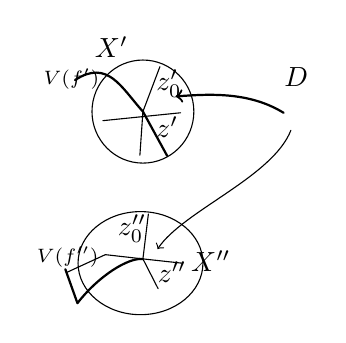
\begin{tikzpicture}[scale=.77,line join=round,line cap=round]
\draw (0,1.5) ellipse (.84 and .85); \node at (-.52,2.56){$X'$};
\draw[thick](-1.12,2.02)..controls(-.58,2.37)and(-.36,1.9)..(0,1.5)--(.4,.77);
\draw (0,1.5)--(.28,2.24) (0,1.5)--(-.05,.78) (-.66,1.35)--(.62,1.48);
\node at (.43,1.96){$z'_0$};\node at (.4,1.25){$z'$};\node at (-1.18,2.04){\scriptsize $V(f')$};
\draw (-.04,-1) ellipse (1.03 and .85); \draw (-1.25,-1.15)--(-.62,-.86)--(0,-.93)--(.64,-1);
\draw[thick](-1.28,-1.1)--(-1.08,-1.66)..controls(-.73,-1.21)and(-.25,-.91)..(0,-.93);
\draw (0,-.93)--(.09,-.19) (0,-.93)--(.25,-1.42);
\node at (-.18,-.43){$z''_0$};\node at (.48,-1.15){$z''$};\node at (1.12,-.96){$X''$};\node at (-1.24,-.9){\scriptsize $V(f'')$};
\node at (2.53,2.07){\uline{$D$}}; \draw[->,thick](2.32,1.48) .. controls (1.75,1.83) and (1.1,1.79) .. (.54,1.75);
\draw[->](2.44,1.19)..controls(2.14,.42)and(.66,-.14)..(.24,-.77);
\end{tikzpicture}}

% manuscript lines 10–11
$D$ un \deleted{\unsure{sous-}}schéma \deleted{fermé de $X$} \inserted{local intègre} de dim $1$

% manuscript lines 12
\deleted{$D'$ \rule{10em}{.35pt} $Y$ de dim $1$}

% manuscript lines 13–14
\[
\left.\begin{aligned}
u' &:D\longrightarrow X'\\
u'' &:D\longrightarrow X''
\end{aligned}\right.\qquad\text{des \uuline{immersions fermées}}
\]

% manuscript lines 15
\[
\underline{u'(D)\not\supset Z'_0}
\]

% manuscript lines 16–20
$X=X'\amalg_D X''$ on identifie $X'$ et $X''$ à des sous-schémas fermés, \unsure{donc} $Z'_0,Z''_0$ aussi. On identifie $D$ à un \deleted{$\unsure{Z}$} ss-schéma fermé \deleted{$\unsure{Z}$} de $X$.

% manuscript lines 17–23
\margin{$A'\times_B A''$\quad $\unsure{f_0}$\quad $\underline{f=(f',f'')}$ \quad $0\longrightarrow C\longrightarrow A'\times A''\xrightarrow{u'-u''}B\longrightarrow0$\quad $(g',g'')\in C$\quad $g'=f'h'$, $g''=f''h''$. $(h',h'')\in C$}
% slanted

% manuscript lines 18–20
\diagram{\begin{tikzcd}[ampersand replacement=\&,row sep=tiny,column sep=small]
\&A'\arrow[r]\& B\\ C\arrow[ur]\arrow[r]\&A''\arrow[ur,dash]\&
\end{tikzcd}}

% manuscript lines 21–23
$f_0\in\deleted{\unsure{H^0}}(\underline O_{D,x})$, $f_0\ne0$. On relève $f_0$ en $f',f''$, d'où $f\in\underline O_{X,x}$ \deleted{est} qui est \uline{non div de $0$} \deleted{\unsure{donc}}. On a
\[
 V(f)\simeq V(f')\amalg_{V(f_0)}V(f'')
\]
% archive sheet number: 91

\scanpage{93}
% manuscript lines 1–2
On suppose alors $V(f')$ et $V(f'')$ sont sans idéaux immergés

% manuscript lines 1–2
\margin{[il ne pourrait y en avoir qu'au pt $x$]}

% manuscript lines 3
[On peut $=$ les prendre intègres]

% manuscript lines 4–5
\[
\begin{aligned}
(V(f)\cap Z'_0={})\ V(f')\cap Z'_0&=\{x\}\\
(V(f)\cap Z''_0={})\ V(f'')\cap Z''_0&\unsure{\subseteq|=|\subset}\{x\}
\end{aligned}
\]

% manuscript lines 6–9
Il s'ensuit que $V(f)$ \uline{est sans} \uline{idéaux} immergés [et $=$ réduit si on veut], et que $V(f)$ est Coh. Mac. en dehors de $\{x\}$.

% manuscript lines 9
\figure{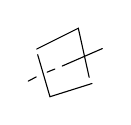
\begin{tikzpicture}[scale=.6,line cap=round]
\draw (.1,.95)--(.98,1.39)--(1.21,.35); \draw (.12,.83)--(.38,-.06)--(1.27,.22);
\draw (-.08,.27)--(.09,.36); \draw[dashed](.32,.46)--(.59,.57); \draw (.64,.59)--(1.49,.96);
\end{tikzpicture}}

% manuscript lines 9–13
\deleted{Donc au pt} Donc l'ens des pts où $X$ n'est pas Coh. Mac. est $Z=\deleted{\unsure{X}}Z'_0\cup Z''_0\cup D$, qui dans $X-V(f)$ est de codim $\leq\operatorname{codim}_{X'}Z'_0<n'\deleted{\unsure{1}}$, [car $Z'_0\ne\varnothing$, $Z'_0\ne\{x\}$], \deleted{et qui dans}

% manuscript lines 14–17
alors que la codim dans $V(f)$ de $V(f)\cap Z$ [i.e. l'ens des pts de $V(f)$ où \deleted{\unsure{Z}} il n'est pas Coh. Mac] est de codim $=\deleted{\unsure{\leq}}\dim V(f)=n''-1\geq n'$.
% archive sheet number: 92

\scanpage{94}
% manuscript lines 1–5
Pour faire la construction \inserted{d'un exemple}, on part d'un \deleted{surface} \inserted{schéma} projectif \inserted{intègre normal} $S'$ \deleted{qui soit \unsure{[donc]}} \inserted{sur un corps alg clos $k$,} qui n'est pas Cohen-Macaulay, \deleted{\unsure{tel qu'on} \unsure{appart} [l'un des} \inserted{[donc de dim $d\geq3$]}

% manuscript lines 6–9
et \unsure{pour|prend} $X'$ le schéma localisé en le sommet du cône projetant de $X'$, $X'$ étant prise \uline{projectivement} \uline{normale}. Donc $n'=d+1\geq4$. \deleted{On prend $X''$ \unsure{une}} On voit que \deleted{\unsure{n}} $Z'_0\ne\varnothing$, $Z'_0\ne\{x\}$ est vérifié.

% manuscript lines 10–14
On prend $X''=$ \deleted{$\unsure{V(k^{n''})}$} localisé en l'origine de $V(k^{n''})$, où \uuline{$n''>n'=d+1$}. Il existe alors un morphisme \inserted{d'imm. \unsure{fermé|fermée} $u'$} de $D=\operatorname{Spec} k[t]_{t k[t]}$ dans $X'$, qui soit tel que \uuline{$u'(D)\not\supset Z'_0$} [prendre une génératrice assez générale],

% manuscript lines 15–16
et on prend une immersion $u'':D\longrightarrow X''$. (par une droite de l'espace affine).

% manuscript lines 17–21
On choisit $f_0$ \unsure{quelc.}, puis $f'$ et $f''$ de façon à vérifier $V(f')\cap Z'_0=\{x\}$, \deleted{\unsure{et}} d'ailleurs $V(f'')\cap Z''_0\subset\{x\}$ est trivial. La \uline{normalité} de $X'$ et $X''$ implique que $V(f')$ et $V(f'')$ n'ont pas d'idéaux immergés \textendash\textendash
% archive sheet number: 93

\scanpage{96}
% manuscript lines 1–3
\uline{Proposition} Soient $K$ anneau, $A,B,C$ des algèbres graduées sur $K$, à \uline{degrés positifs}, et réduites à $K$ en degré $0$,

% manuscript lines 1–6
% slanted
\margin{\unsure{Comparer aux} développements des ``\uline{immersions régulières}'' \uline{Modules} [quand on a un $B$-module $M$]}

% manuscript lines 4
\diagram{\begin{tikzcd}[ampersand replacement=\&]
A\arrow[r,"\psi"]\&B\arrow[r,"\varphi"]\&C
\end{tikzcd}}

% manuscript lines 5
des homomorphismes. On suppose

% manuscript lines 6–8
a) Pour tt $i\geq0$, $\varphi^i:B^i\longrightarrow C^i$ est surjectif et admet un hom inverse à gauche $K$-linéaire, soit $u^i:C^i\longrightarrow B^i$

% manuscript lines 9–10
\textcircled{1} Alors les conditions b) et b') suivantes sont équivalentes

% manuscript lines 11
b) \deleted{$\varphi$ est surjectif, et} $\operatorname{Ker}\varphi=\psi(A^+)B$

% manuscript lines 11–15
% slanted
\margin{N.B. [Sous a)] Si $A$ engendré par $A^1$, alors b) équivaut à $\operatorname{Ker}\varphi=\psi(A^1).B$ i.e. b$_1$) $\operatorname{Ker}\varphi^1=\psi^1(A^1)$ b$_2$) $\operatorname{Ker}\varphi$ engendré par $\operatorname{Ker}\varphi^1$}

% manuscript lines 12–13
b') Pour tt $n\geq0$, l'hom
\[
v^n:\sum_{i+j=n}\unsure{A^i|A_i}\otimes_K C^j\longrightarrow B^n
\]

% manuscript lines 14–17
\deleted{de composantes \unsure{$(a$}} tel que
\[
 v^n(a^i\otimes c^j)=\psi(a^i)\deleted{\unsure{\otimes}}u^j(c^j)
\]
est \uline{surjectif}.

% manuscript lines 18–19
[Donc (b') ne dépend pas des choix des $u^j$].
% archive sheet number: 95

\scanpage{97}
% manuscript lines 1–2
\textcircled{2} Supposons qu'on ait $=$
\[
\text{b'')}\qquad v^n\ \text{est bijectif}
\]

% manuscript lines 3–6
Alors $\psi$ est \uline{injectif}. \deleted{Alors} De plus, les $B^i$ sont plats [resp. \deleted{libres,} projectifs] sur $K$ sss les $A^i,C^i$ le sont.

% manuscript lines 2–11
% slanted
\margin{\uline{N.B.} On devrait vérifier que (b'') ne dépend pas du choix des $u^n$. [Si les $A^i,B^i$ de type fini, celà se ramène au cas d'un corps de base, (comme dans $3^\circ$) grâce à Nakayama]}

% manuscript lines 7–10
\textcircled{3} \deleted{Réciproquement, supposons \deleted{\unsure{les|que}} les $A^i,B^i,C^i$ projectifs de type fini [= plats de présentation finie]} Pour tt $x\in\operatorname{Spec} K$, soit

% manuscript lines 11
\[
 P_{A,x}\deleted{\unsure{A}}(t)=\sum\operatorname{rg}_{k(x)}(A^i(x))t^i\in\mathbb Z[[t]]
\]

% manuscript lines 12–13
et définissons de $=$ $P_{B,x}(t)$, $P_{C,x}(t)$. Alors on a \deleted{\unsure{tt}} pour tt $x$ [moyennant a]

% manuscript lines 14
\[
P_{B,x}\ll P_{A,x}\,P_{C,x}\tag*{\textcircled{*}}
\]

% manuscript lines 15–18
[majoration coefficient par coefficient]. Si (b'') est vérifié, alors on a $=$

% manuscript lines 16–17
\margin{c) $P_{B,x}=P_{A,x}P_{C,x}$}

% manuscript lines 17–19
Si les $A^i,B^i,C^i$ sont plats de prés. finie [= projectifs de type fini], alors c) implique aussi b''), \deleted{donc \unsure{Donc}}
% archive sheet number: 96

\scanpage{98}
% manuscript lines 1
\uline{Corollaire 1} Conditions équivalentes \inserted{moyennant a)}

% manuscript lines 2
(i) $v^*$ bijectif, les $B^i$ projectifs de type fini

% manuscript lines 3
(ii) $v^*$ bijectif, les $A^i,C^i$ projectifs de type fini

% manuscript lines 4–5
(iii) les $A^i,B^i,C^i$ projectifs de type fini, \deleted{et} $P_{B,x}=P_{A,x}P_{C,x}$ pour tt $x$.

% manuscript lines 6–7
[N.B. Si $K$ est local, il suffit de regarder en le pt fermé].

% manuscript lines 8–12
\uline{N.B.} Nous référerons à l'ens des conditions a), b'') comme ``bonnes'', si de plus les $B^i$ sont projectifs de type fini, on dira ``très bonnes''.

% manuscript lines 13–17
\uline{Question} Sous les ``bonnes conditions'' prouver
\[
\begin{aligned}
\text{(i)}\quad &A\ \text{plat}/K\Longrightarrow C\ \text{plat}/B\\
\text{(ii)}\quad &C\ \text{plat}/K\Longrightarrow B\ \text{plat}/A\\
\text{donc}\qquad\text{(iii)}\quad &A\text{ et }C\ \text{plats}/K\Longrightarrow B\ \text{plat}/K
\end{aligned}
\]
% archive sheet number: 97

\scanpage{99}
% manuscript lines 1–3
\uline{Corollaire} 2 Supposons que $C\simeq K[t_1,\text{--},t_r]$, les $t_i$ homogènes \inserted{[néc de degr $>0$]}. Alors $(a,b'')$ équivaut à ceci :

% manuscript lines 4–8
\[
\left\{\begin{aligned}
 B&\simeq A[t_1,\text{--}t_r]\\
 \psi&\simeq\text{hom can}\quad A\longrightarrow A[t_1,\text{--}t_r]\\
 \varphi&\simeq\text{hom passage au quotient}\\
 &\qquad A[t_1,\text{--},t_r]\longrightarrow\underbrace{A/A^+}_{K}[t_1,\text{--}t_r]
\end{aligned}\right.
\]

% manuscript lines 9–13
[Le choix d'un isom $B\simeq A[t_1,\text{--}t_r]$ équivaut à celui d'un \uline{hom} \uline{d'alg} \deleted{\unsure{d'une|d'un}} $\underline{C\xrightarrow{u}B}$ tel que $\varphi u=\mathrm{id}_C$, ou encore d'un hom $K$-linéaire qui relève $B^+\longrightarrow C^+/C^{+2}$].
% archive sheet number: 98

